\documentclass{../../td}{subfiles}
\usepackage{../../raccourcis}
\begin{document}
\subsection*{Exercice I : Gain complexe équivalent}
\begin{enumerate}\setlength{\itemsep}{1cm}
\newcommand\conftitle{some conference}
\item Pour la fonction de seuil:
%\img{0.5}{1.png}
\[ y = 
\left\{
\begin{array}{cc}
0 & \text{ si } |X| \leq \frac{\Delta}{2} \\
x-\frac{\Delta}{2} & \text{ si } X > \frac{\Delta}{2} \\
x+\frac{\Delta}{2} & \text{ si } X < -\frac{\Delta}{2}
\end{array}
\right.
\]


%\img{0.5}{2.png}

		On pose \[ N(X) = \frac{P+jQ}{X} \] avec \[ Q=0 \]
\begin{align*}
P &= \frac{4\omega}{\pi} \int_{t_1}^{\frac{\pi}{2\omega}}(Xsin(\omega t) - \frac{\Delta}{2})sin(\omega t) dt\\
&= \frac{4\omega}{\pi} \int_{t_1}^{\frac{\pi}{2\omega}}(Xsin^2(\omega t) - \frac{\Delta}{2}sin(\omega t)) dt\\
&=-\frac{2\Delta}{\pi}cos(\omega t_1) - \frac{4 X \omega}{\pi}(\frac{t_1}{2} - \frac{\pi}{4\omega} - \frac{sin(2t_1 \omega}{4\omega})\\
\text{Or, } & Xsin(\omega t_1) = \frac{\Delta}{2} \Rightarrow t_1 = \frac{1}{\omega} arcsin(\frac{\Delta}{2X})\\
&\Rightarrow P = X (1 -  \frac{2}{\pi}(arcsin(\frac{\Delta}{2X}) + \frac{\Delta}{2X}\sqrt{1-(\frac{\Delta}{2X})^2}
\end{align*}

On a alors $N(X) = \frac{P}{X}$.


\item Pour le relais avec hystérésis

%\img{0.5}{3}
On pose $X\sin(\omega t_1) = \frac{h}{2} \text{ donc } t_1 = \frac{1}{\omega} arcsin(\frac{h}{2X})$

\begin{figure}[h!]
\centering
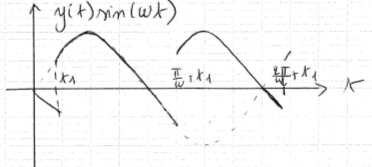
\includegraphics[scale=0.5]{4}
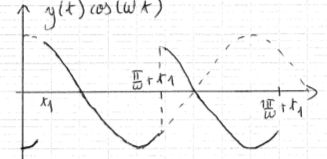
\includegraphics[scale=0.5]{5}
\end{figure}

\begin{multicols}{2}
\begin{align*}
P & = \frac{\omega}{\pi} \int_{[T]} y(t) \sin(\omega t) dt \\
& = 2\frac{\omega}{\pi} \int_{t_1}^{\frac{\pi}{\omega}+t_1} M \sin(\omega t) dt\\
& = 2\frac{\omega}{\pi}M . \frac{-\cos(\pi+\omega t_1) + \cos(\omega t_1)}{\omega} \\ 
P & = \frac{4M}{\pi} \sqrt{1-(\frac{h}{2X})^2}
\end{align*}

\begin{align*}
Q & = \frac{\omega}{\pi} \int_{[T]} y(t) \cos(\omega t) dt \\
& = 2\frac{\omega}{\pi} \int_{t_1}^{\frac{\pi}{\omega}+t_1} M \cos(\omega t) dt \\
& = 2\frac{\omega}{\pi}M.\frac{\sin(\pi + \omega t_1) - \sin(\omega t_1)}{\omega} \\
Q & = -\frac{4M}{\pi} \frac{h}{2X}
\end{align*}
\end{multicols}

\[ |N(X)| = \frac{\sqrt{P^2 + Q^2}}{X} = \frac{4M}{\pi X} \]

\item Pour le jeux sans inertie aval
%\img{0.5}{6}

\[ y(t) = 
\left\{
\begin{array}{cc}
x(t) - \alpha & \text{ sur } DA\\
M & \text{ sur } AB \\
x(t) + \alpha & \text{ sur } BC \\
-M & \text{ sur } CD
\end{array}
\right.
\]

\[ |N(X)| = \frac{1}{2\pi}\sqrt{ (1+\cos2\beta)^2 - (\pi+2\beta+\sin2\beta)^2} \avec \beta = \arcsin(1-2\frac{\alpha}{M}) \]

\end{enumerate}

\subsection*{Exercice II : Asservissement avec boucle secondaire}

\begin{enumerate}\setlength{\itemsep}{1cm}

\item Relations entre les différentes variables
\begin{align*}
s(p(1+T_2p)) = k_2 w & \Rightarrow \dd{s}{t} + T_2 \dd{^2 s}{t^2} = k_2 w(t) \\
w = \phi(x) & \\
x = r - ks & \\
r(1+T_1 p) = -k_1 s & \Rightarrow r(t) + T_1 \dd{r}{t} = -k_1 s(t)
\end{align*}

\item On exprime $x$ en fonction de $s$ et $s$ en fonction de $x$ :
\begin{align*}
x & = \frac{-k_1}{1+T_1 p} s - ks \\
s & = \frac{k_2}{p(1+T_2p)}\phi(x)
\end{align*}
donc
\[ p(1+T_2p)(1+T_1p)x = -(k_1+k(1+T_1p))k_2\phi(x) \]
\[ T_2T_1x^{(3)} + (T_1+T_2)x^{(2)} + x^{(1)} = -k_2(k_1+k)\phi(x)-kk_2T_1 \dd{\phi(x)}{t} \]

\item On peut appliquer l'approximation du 1er harmonique à la NL car :
\begin{itemize}
\item La NL est statique
\item Un filtre passe-bas d'ordre relatif $>1$ est en aval de la NL
Si le filtre est $\frac{p+1}{p^2 / \omega^2 + 2m/\omega p +1}$, on ne peut pas appliquer la méthode du 1er harmonique.

\end{itemize}

\item On a $Q=0$ car la NL est impaire.
\[ P = \frac{2}{T} \int_0^T y(t) \sin(\omega t) dt = \frac{2}{T} ( \int_0^{T/2} M\sin (\omega t) dt - \int_{T/2}^T M\sin(\omega t) dt) = \frac{4M}{\pi} \]

\item Avec $x(t)=X\sin(\omega t)$, on a donc l'approximation $w(t)=N(X).x(t)$ avec $N(x)=\frac{4M}{\pi X}$.

\item Analyse harmonique en remplaçant $\frac{d}{dt}=j\omega$
\[ -T_1T_2 j\omega^3 - (T_1+T_2) \omega^2 + j(1+kk_2T_1N(X)) \omega + (k_1+k)k_2N(X) = 0 \]

On en déduit les équations algébriques du cycle limite en prenant parties réelle et imaginaire :
\begin{align*}
(k_1+k)k_2 N(X)  - (T_1+T_2) \omega^2 & = 0 \\
(1+kk_2T_1N(x))\omega - T_1T_2 \omega^3 & =0
\end{align*}

\item Cycle limite.\\

\paragraph{Existence du cycle limite} On cherche une solution aux équations algébriques :
\begin{align*}
Re=0 & \Rightarrow \omega_0^2 = \frac{(k_1+k)k_2N(x)}{T_1+T_2} \\
Im=0 & \Rightarrow X_0 = \frac{4Mk_2T_1(k_1T_2-kT_1)}{\pi(T_1+T_2)}
\end{align*}

On peut alors réécrire \[\omega_0^2 = \frac{k_1+k}{T_1(k_1T_2-kT_1)} \]

\paragraph{Stabilité du cycle limite}
\[ \derivp[R]{X}|_0 \derivp[I]{\omega}|_0 - \derivp[I]{X}|_0 \derivp[R]{\omega}|_0 > 0 \]

\begin{align*}
\derivp[R]{X}|_0 & = (k+k_1)k_2 \dd{N}{X}|_0 < 0 \\
\derivp[R]{\omega}|_0 & = -2(T_1+T_2)\omega_0 < 0 \\
\derivp[I]{X}|_0 & = kk_2T_1 \dd{N}{X}|_0 \omega_0< 0 \\
\derivp[I]{\omega}|_0 & = 1 + kk_2T_1N(X_0)-3T_1T_2\omega_0 = -2T_1T_2\omega_0^2 < 0
\end{align*}

Le cycle limite est stable si $\derivp[R]{X}|_0 \derivp[I]{\omega}|_0 - \derivp[I]{X}|_0 \derivp[R]{\omega}|_0 > 0$
\[-2(k+k_1)k_2\dd{N}{X}T_1T_2\omega_0^2 + 2(T_1+T_2)\omega_0^2kk_2T_1\dd{N}{X}> 0\]

soit
\[T_2(k+k_1)\dd{N}{X}|_0 + (T_1+T_2)k\dd{N}{X}|_0 > 0\]

soit \[T_1k-T_2k_1<0\]

Même condition que celle d'existence du cycle limite.

%\img{0.5}{7}
\end{enumerate}


\subsection*{Exercice III : Contre-exemple}

\begin{enumerate}\setlength{\itemsep}{1cm}

\item Voir Exercice I :
\[ N(x) = \frac{4M}{\pi X}\sqrt{1-(\frac{h}{2X})^2} - j\frac{2Mh}{\pi X^2} = N_P(x) + jN_Q(X) \quad \et \quad |N(X)| = \frac{4M}{\pi X}\]

Le lieu critique est défini par 
\[ - \frac{1}{N(x)} = \frac{-N_P(X) + j N_Q(X)}{|N(X)|^2} = -\frac{\pi X}{4M}\sqrt{1-(\frac{h}{2X})^2} - j\frac{\pi^2h}{8M} \]

On trace le lieu de Nyquist de la fonction de transfert de $\frac{K}{1+\tau p}$ ainsi que celui de $-\frac{1}{N(X)}$ :

%\img{0.5}{8}

Il n'y a pas d'intersection entre les deux : d'après la méthode du 1er harmonique, il n'y a donc pas de cycle limite.

\item $KM > h/2$

L'entrée du filtre du 1er ordre $u=M$

\[y(t) = KM(1-e^{-t/\tau}) \Rightarrow \exists t_1 \text{ tq } y(t_1) > h/2 \text{ car } KM>h/2 \]
\[x(t) = -y(t) < -h/2 \Rightarrow u = -M\]

et avec le même raisonnement,
\[ \exists t_2 \text{ tq } y(t_2) < -h/2 \]
\[ x(t) > h/2 \]

donc pour $KM>h/2$, il existe un cycle limite.

\item On obtient une contradiction car le filtre est de degré relatif égal à 1.
\end{enumerate}

\end{document}
